%%%%%%%%%%%%%%%%%%%%%%%%%%%%%%%%%%%%%%%%%
% Beamer Presentation
% LaTeX Template
% Version 1.0 (10/11/12)
%
% This template has been downloaded from:
% http://www.LaTeXTemplates.com
%
% License:
% CC BY-NC-SA 3.0 (http://creativecommons.org/licenses/by-nc-sa/3.0/)
%
%%%%%%%%%%%%%%%%%%%%%%%%%%%%%%%%%%%%%%%%%

%----------------------------------------------------------------------------------------
%	PACKAGES AND THEMES
%----------------------------------------------------------------------------------------

\documentclass{beamer}

\mode<presentation> {

% The Beamer class comes with a number of default slide themes
% which change the colors and layouts of slides. Below this is a list
% of all the themes, uncomment each in turn to see what they look like.

%\usetheme{default}
%\usetheme{AnnArbor}
%\usetheme{Antibes}
%\usetheme{Bergen}
%\usetheme{Berkeley}
%\usetheme{Berlin}
%\usetheme{Boadilla}
%\usetheme{CambridgeUS}
%\usetheme{Copenhagen}
\usetheme{Darmstadt}
%\usetheme{Dresden}
%\usetheme{Frankfurt}
%\usetheme{Goettingen}
%\usetheme{Hannover}
%\usetheme{Ilmenau}
%\usetheme{JuanLesPins}
%\usetheme{Luebeck}
%\usetheme{Madrid}
%*\usetheme{Malmoe}
%\usetheme{Marburg}
%\usetheme{Montpellier}
%\usetheme{PaloAlto}
%\usetheme{Pittsburgh}
%\usetheme{Rochester}
%\usetheme{Singapore}
%\usetheme{Szeged}
%\usetheme{Warsaw}

% As well as themes, the Beamer class has a number of color themes
% for any slide theme. Uncomment each of these in turn to see how it
% changes the colors of your current slide theme.

%\usecolortheme{albatross}
%\usecolortheme{beaver}
%\usecolortheme{beetle}
%\usecolortheme{crane}
%\usecolortheme{dolphin}
%\usecolortheme{dove}
%\usecolortheme{fly}
%\usecolortheme{lily}
\usecolortheme{orchid}
%\usecolortheme{rose}
%\usecolortheme{seagull}
%\usecolortheme{seahorse}
%\usecolortheme{whale}
%\usecolortheme{wolverine}

%\setbeamertemplate{footline} % To remove the footer line in all slides uncomment this line
%\setbeamertemplate{footline}[page number] % To replace the footer line in all slides with a simple slide count uncomment this line

%\setbeamertemplate{navigation symbols}{} % To remove the navigation symbols from the bottom of all slides uncomment this line
}


\usepackage{graphicx} % Allows including images
\usepackage{booktabs} % Allows the use of \toprule, \midrule and \bottomrule in tables
\usepackage{xspace}
\usepackage{caption}
\usepackage{subfigure}
\usepackage[english,brazil]{babel}
\usepackage[utf8]{inputenc}

%Renomeia o nome padrao das figuras.
\renewcommand{\figurename}{Figura}
\renewcommand{\tablename}{Tabela}



\usepackage[pygopt={texcomments=true,style=emacs}]{pythontex}
\setpythontexlistingenv{listing}

\newcounter{sublisting}[listing]
\newcommand{\codeline}[1]{%
  \addcontentsline{lopytx}{listing}%
    {\protect\numberline{\hspace{0.5in}\thelisting.\arabic{FancyVerbLine}}\hspace{0.5in}#1}%
}


%----------------------------------------------------------------------------------------
%	TITLE PAGE
%----------------------------------------------------------------------------------------

\title[Computação Gráfica]{Determinação de Superfícies Visíveis} % The short title appears at the bottom of every slide, the full title is only on the title page

\author{Uéliton Freitas} % Your name
\institute[UFMS] % Your institution as it will appear on the bottom of every slide, may be shorthand to save space
{
Universidade Católica Dom Bosco - UCDB \\ % Your institution for the title page
\medskip
\textit{freitas.ueliton@gmail.com} % Your email address
}
\date{\today} % Date, can be changed to a custom date


\begin{document}

\begin{frame}
\titlepage % Print the title page as the first slide
\end{frame}

\begin{frame}
\frametitle{Sumário} % Table of contents slide, comment this block out to remove it
\tableofcontents % Throughout your presentation, if you choose to use \section{} and \subsection{} commands, these will automatically be printed on this slide as an overview of your presentation
\end{frame}




%----------------------------------------------------------------------------------------
%	PRESENTATION SLIDES
%----------------------------------------------------------------------------------------

%------------------------------------------------
\section{Introdução} 
%------------------------------------------------

%\section{Speeded-Up Robust Features - SURF} % A subsection can be created just before a set of slides with a common theme to further break down your presentation into chunks
%\section{Baf Of Features and Colors}

%\section{Refer\^encias}
%%%%%%%%%%%%%%%%%%%%%%%%%%%%%%%%%%%%%%%%%%%%%%%%%%%%%%%%%%%%%%%%%%%%%%%%%%%%%%%%%%%%%%%%%%
\begin{frame}
\frametitle{Introdução}

		\begin{block}{Rendering de Polígonos}
			\begin{itemize}
				\item Por eficiência, queremos renderizar apenas as faces poligonais que são visíveis para a câmera.
			\end{itemize} 
		\end{block}
		\begin{block}{}
			\begin{itemize}
				\item Existem diversos algoritmos para \textbf{detecção de superfícies visíveis} (ou eliminação de superfícies ocultas) que variam conforme:
				\begin{itemize}
					\item Complexidade da cena.
					\item Tipo de objeto desenhado.
					\item Equipamento disponível.
					\item etc. 
				\end{itemize}
			\end{itemize} 
		\end{block}
	
\end{frame}


%%%%%%%%%%%%%%%%%%%%%%%%%%%%%%%%%%%%%%%%%%%%%%%%%%%%%%%%%%%%%%%%%%%%%%%%%%%%%%%%%%%%%%%%%%
\begin{frame}
\frametitle{Introdução}

		\begin{block}{Classificação dos Algoritmos}
			\begin{itemize}
				\item Os algoritmos podem ser classificados em dois grandes grupos:
					\begin{itemize}
						\item Métodos de \textbf{espaço do objeto}.
						\item Métodos de \textbf{espaço da imagem}.
					\end{itemize}
			\end{itemize} 
		\end{block}
		
		\begin{block}{Espaço do Objeto}
			\begin{itemize}
				\item Compara objetos entre si, ou partes de objetos, para determinar a visibilidade.
			\end{itemize}
		\end{block}

		\begin{block}{Espaço da Imagem}
			\begin{itemize}
				\item Compara pixel por pixel no plano de projeção para determinar a visibilidade.
			\end{itemize}
		\end{block}
\end{frame}

%%%%%%%%%%%%%%%%%%%%%%%%%%%%%%%%%%%%%%%%%%%%%%%%%%%%%%%%%%%%%%%%%%%%%%%%%%%%%%%%%%%%%%%%%%
\begin{frame}
\frametitle{Introdução}

		\begin{block}{Classificação dos Algoritmos}
			\begin{itemize}
				\item Discutiremos dois algoritmos de visibilidade:
					\begin{itemize}
						\item Back-face culling.
						\item Z-buffer.
					\end{itemize}
			\end{itemize} 
		\end{block}
\end{frame}


%%%%%%%%%%%%%%%%%%%%%%%%%%%%%%%%%%%%%%%%%%%%%%%%%%%%%%%%%%%%%%%%%%%%%%%%%%%%%%%%%%%%%%%%%%
\section{Back-Face Culling}
\begin{frame}
\frametitle{Back-Face Culling}

		\begin{block}{Back-Face Culling}
			\begin{itemize}
				\item Se as faces pertencem a um objeto sólido (um poliedro, por exemplo), não é necessário renderizar as faces de trás (não visíveis).
			\end{itemize} 
		\end{block}
		
		\begin{figure}[!h]
			\begin{center}
				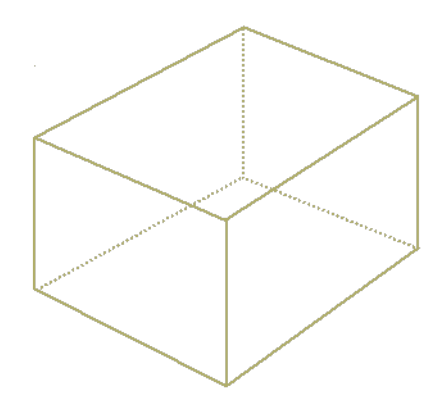
\includegraphics[width=0.3\textwidth]{Figures/Cub}
			\end{center}
		\end{figure}
		
\end{frame}


%%%%%%%%%%%%%%%%%%%%%%%%%%%%%%%%%%%%%%%%%%%%%%%%%%%%%%%%%%%%%%%%%%%%%%%%%%%%%%%%%%%%%%%%%%
\begin{frame}
\frametitle{Back-Face Culling}

		\begin{figure}[!h]
			\begin{center}
				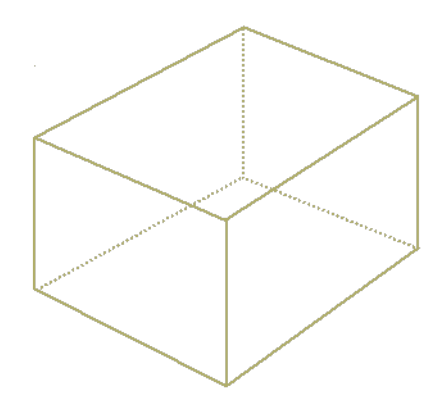
\includegraphics[width=0.3\textwidth]{Figures/Cub}
			\end{center}
		\end{figure}
		
		\begin{block}{Back-Face Culling}
			\begin{itemize}
				\item Apenas três faces precisam ser traçadas.
			\end{itemize}
		\end{block}
		
		\begin{block}{}
			\begin{itemize}	
				\item As faces ``de trás'' podem ser removidas do pipeline. 
			\end{itemize}
		\end{block}
		
\end{frame}

%%%%%%%%%%%%%%%%%%%%%%%%%%%%%%%%%%%%%%%%%%%%%%%%%%%%%%%%%%%%%%%%%%%%%%%%%%%%%%%%%%%%%%%%%%
\begin{frame}
\frametitle{Back-Face Culling}

		\begin{figure}[!h]
			\begin{center}
				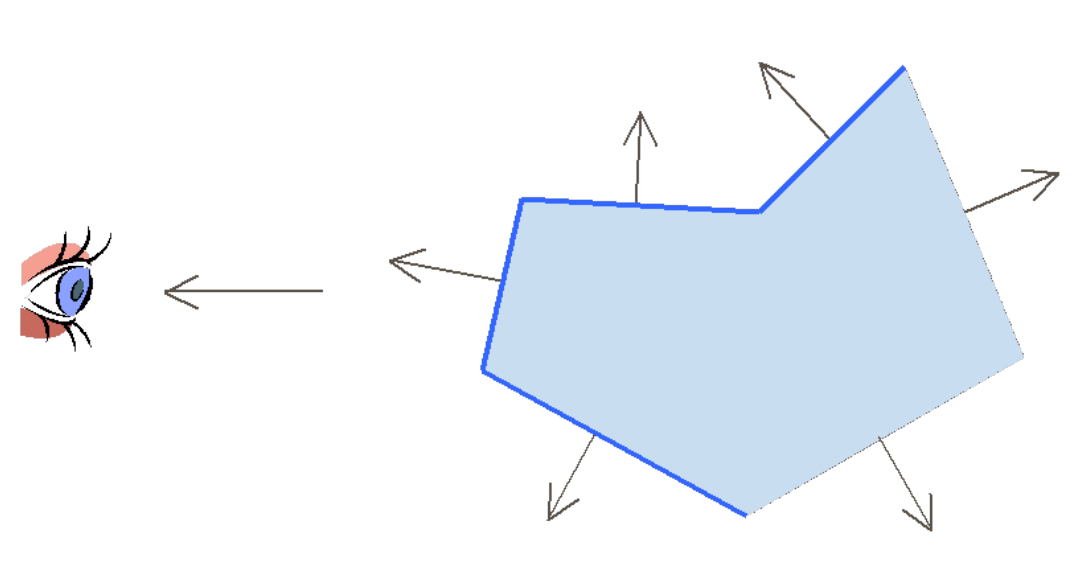
\includegraphics[width=0.8\textwidth]{Figures/FroFac}
			\end{center}
		\end{figure}
		
		\begin{block}{Back-Face Culling}
			\begin{itemize}	
				\item Assume-se que a cena é composta por poliedros fechados.
			\end{itemize}
		\end{block}
		
\end{frame}

%%%%%%%%%%%%%%%%%%%%%%%%%%%%%%%%%%%%%%%%%%%%%%%%%%%%%%%%%%%%%%%%%%%%%%%%%%%%%%%%%%%%%%%%%%
\begin{frame}
\frametitle{Back-Face Culling}

		\begin{block}{Back-Face Culling}
			\begin{itemize}	
				\item Como descobrir quais são as ``faces de trás''?
			\end{itemize}
		\end{block}


		\begin{figure}[!h]
			\begin{center}
				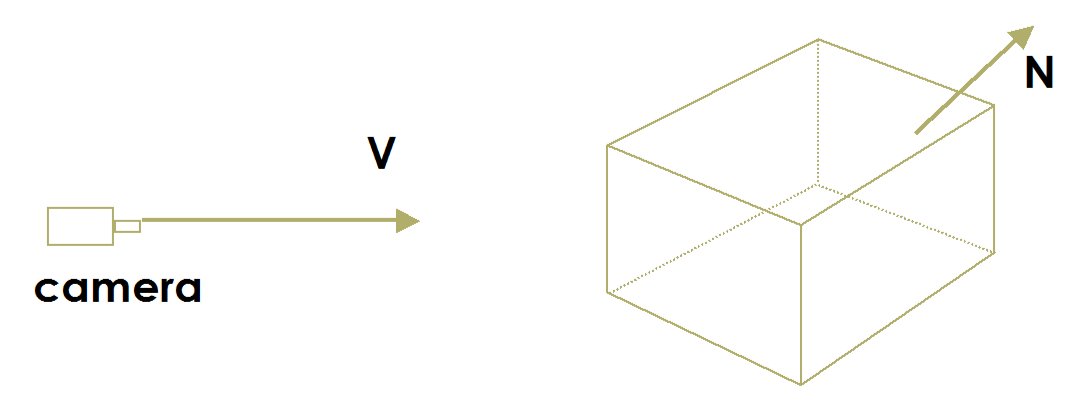
\includegraphics[width=0.8\textwidth]{Figures/CamCub}
			\end{center}
		\end{figure}
		
\end{frame}

%%%%%%%%%%%%%%%%%%%%%%%%%%%%%%%%%%%%%%%%%%%%%%%%%%%%%%%%%%%%%%%%%%%%%%%%%%%%%%%%%%%%%%%%%%
\begin{frame}
\frametitle{Back-Face Culling}

		\begin{block}{Back-Face Culling}
			\begin{itemize}	
				\item Uma \textbf{face} é uma face de ``faces de trás'' (não visível) de um polígono se o \textbf{ângulo} entre o vetor normal a face \textbf{N} e o vetor direção de observação \textbf{V} é \textbf{menor do que} $90^\circ $.\\
				\begin{equation*}
					V \cdot N > 0
				\end{equation*}				 
			\end{itemize}
		\end{block}


		\begin{figure}[!h]
			\begin{center}
				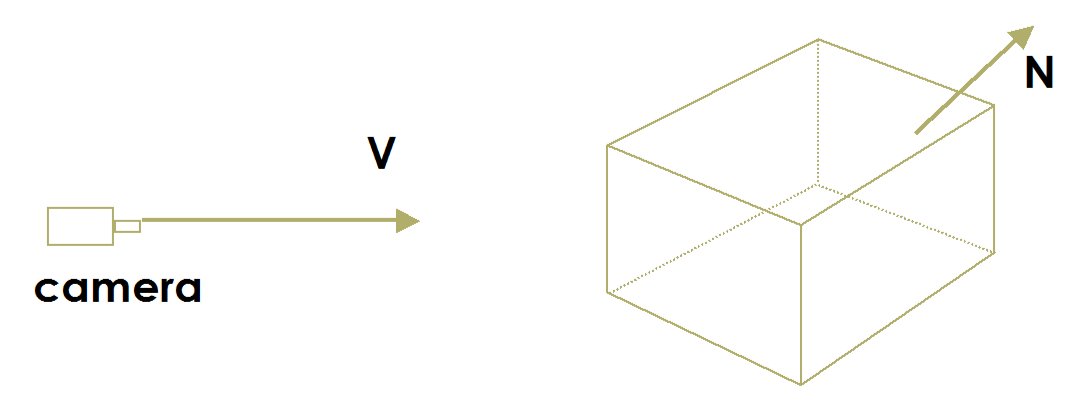
\includegraphics[width=0.8\textwidth]{Figures/CamCub}
			\end{center}
		\end{figure}
		
\end{frame}


%----------------------------------------------------------------------------------------
\end{document} 